\documentclass[11pt]{article}
 
\usepackage[top=0.75in, bottom=1.25in, left=1in, right=1in]{geometry} 
\usepackage{amsmath,amsthm,amssymb} %this is THE math package
\usepackage{mathtools}
\usepackage{tikz}
\usepackage{graphicx}
\usepackage{fancybox}
\usepackage{hyperref}
\usepackage{varwidth}
\usepackage{mdframed}
\usepackage{mathrsfs}
\usepackage[most]{tcolorbox}
%------------------------
%Fonts I use, uncomment if you like to use them.
%The first is the general font, and the second a math font
\usepackage{mathpazo}
\usepackage{eulervm}
%------------------------
%This is so that we have standard fonts for the double-stroked symbols
%for reals, naturals etc. regardless of what font you use.
%Don't comment
\AtBeginDocument{
  \DeclareSymbolFont{AMSb}{U}{msb}{m}{n}
  \DeclareSymbolFontAlphabet{\mathbb}{AMSb}}
%------------------------
\usepackage{graphicx}
\graphicspath{ {./images/} }

%----------------------------------------------
%User-defined environments
%Commented because we're not using them in this document
%The only uncommented ones are the Problem and Solution environment

% \newenvironment{theorem}[2][Theorem]{\begin{trivlist}
% \item[\hskip \labelsep {\bfseries #1}\hskip \labelsep {\bfseries #2.}]}{\end{trivlist}}
% \newenvironment{lemma}[2][Lemma]{\begin{trivlist}
% \item[\hskip \labelsep {\bfseries #1}\hskip \labelsep {\bfseries #2.}]}{\end{trivlist}}
% \newenvironment{exercise}[2][Exercise]{\begin{trivlist}
% \item[\hskip \labelsep {\bfseries #1}\hskip \labelsep {\bfseries #2.}]}{\end{trivlist}}
% \newenvironment{question}[2][Question]{\begin{trivlist}
% \item[\hskip \labelsep {\bfseries #1}\hskip \labelsep {\bfseries #2.}]}{\end{trivlist}}
% \newenvironment{corollary}[2][Corollary]{\begin{trivlist}
% \item[\hskip \labelsep {\bfseries #1}\hskip \labelsep {\bfseries #2.}]}{\end{trivlist}}
\newenvironment{problem}[2][Problem\!]{\begin{trivlist}
\item[\hskip \labelsep {\bfseries #1}\hskip \labelsep {\bfseries #2}]}{\end{trivlist}}
%\newenvironment{sub-problem}[2][]{\begin{trivlist}
%\item[\hskip \labelsep {\bfseries #1}\hskip \labelsep {\bfseries #2}]}{\end{trivlist}}
\newenvironment{solution}{\begin{proof}[\textbf{\textit{Solution}}] }{\end{proof}}
%----------------------------------------------

%----------------------------
%User-defined notations
\newcommand{\zz}{\mathbb Z}   %blackboard bold Z
\newcommand{\qq}{\mathbb Q}   %blackboard bold Q
\newcommand{\ff}{\mathbb F}   %blackboard bold F
\newcommand{\rr}{\mathbb R}   %blackboard bold R
\newcommand{\nn}{\mathbb N}   %blackboard bold N
\newcommand{\cc}{\mathbb C}   %blackboard bold C
\newcommand{\af}{\mathbb A}   %blackboard bold A
\newcommand{\pp}{\mathbb P}   %blackboard bold P
\newcommand{\id}{\operatorname{id}} %for identity map
\newcommand{\im}{\operatorname{im}} %for image of a function
\newcommand{\dom}{\operatorname{dom}} %for domain of a function
\newcommand{\cat}[1]{\mathscr{#1}}   %calligraphic category
\newcommand{\abs}[1]{\left\lvert#1\right\rvert} %for absolute value
\newcommand{\norm}[1]{\left\lVert#1\right\rVert} %for norm
\newcommand{\modar}[1]{\text{ mod }{#1}} %for modular arithmetic
\newcommand{\set}[1]{\left\{#1\right\}} %for set
\newcommand{\setp}[2]{\left\{#1\ \middle|\ #2\right\}} %for set with a property
\newcommand{\card}[1]{\#\,{#1}} %for cardinality of a set
\newcommand\m[1]{\begin{pmatrix}#1\end{pmatrix}} 

%Re-defined notations
\renewcommand{\epsilon}{\varepsilon}
\renewcommand{\phi}{\varphi}
\renewcommand{\emptyset}{\varnothing}
\renewcommand{\geq}{\geqslant}
\renewcommand{\leq}{\leqslant}
\renewcommand{\Re}{\operatorname{Re}}
\renewcommand{\Im}{\operatorname{Im}}
%----------------------------

\allowdisplaybreaks
 
 
\begin{document}
 
\title{Assignment}
\author{Kevin Guillen\\[0.5em]
MATH  | Class | Quarter}
\date{} 
\maketitle
%--------------IC SUBMISSION-----------------------------
\begin{tcolorbox}
    \begin{problem}{1}
    Find the sum of:
    \[\frac{1}{1 \cdot 2\cdot 3} + \frac{1}{2 \cdot 3 \cdot 4} + \dots + \frac{1}{100 \cdot 101 \cdot 102}\]
    \end{problem}
    \textbf{Arithmetic and geometric sequences and series} Uses common properties of summation of terms 
\end{tcolorbox}
\begin{solution}
    If we look at this as a summation we can describe each term as, 
    \[\frac{1}{i \cdot (i +1) \cdot (i+2)} \] 
    for $i\in \set{1, \dots, n}$. Giving us,
    \[\sum_{i=1}^n \frac{1}{i \cdot (i +1) \cdot (i+2)}\]
    Doing some algebra we can obtain the following,
    \begin{align*}
        \sum_{i=1}^n \frac{1}{i \cdot (i +1) \cdot (i+2)} &= \sum_{i=1}^n \frac{1}{2}\cdot \frac{2}{i \cdot (i +1) \cdot (i+2)} \\
        &= \frac{1}{2} \cdot \sum_{i=1}^n \frac{i + 2 - i}{i \cdot (i +1) \cdot (i+2)} \\
        &= \frac{1}{2} \cdot\sum_{i=1}^n  \frac{(i + 2)}{i \cdot (i +1) \cdot (i+2)} - \frac{i}{i \cdot (i +1) \cdot (i+2)} \\
        &= \frac{1}{2} \cdot\sum_{i=1}^n  \frac{1}{i \cdot (i +1)} - \frac{1}{(i +1) \cdot (i+2)}
    \end{align*}
    
    \noindent Finally when we expand the summation out we can see something important,
    \[\frac{1}{2}\left(\frac{1}{1 \cdot (2)} - \frac{1}{(2)\cdot(3)} + \frac{1}{2\cdot(3)} - \frac{1}{(3)\cdot(4)}+ \dots + \frac{1}{n \cdot(n+1)}-\frac{1}{(n +1)\cdot(n + 2)}\right)\]
    that the middle terms cancel out giving us,
    \[\frac{1}{2} \cdot \left(\frac{1}{1\cdot(1+1)} - \frac{1}{(n+1)\cdot(n+2)}\right)\]
    Now plugging in our desired value for the problem, $n = 100$, we get,
    \begin{align*}
        \frac{1}{2} \cdot \left(\frac{1}{2} - \frac{1}{101 \cdot 102} \right) &= \frac{1}{4} - \frac{1}{20604} \\ 
        &= \frac{5151}{20604} - \frac{1}{20604}  \\
        &= \frac{5150}{20604}
    \end{align*}
\end{solution}

\begin{tcolorbox}
    \begin{problem}{IC | 9/29 | 14.}
        Let $x$ be a real number such that $x + \frac{1}{x}$ is an integer. Prove $x^n + \frac{1}{x^n}$ is an integer for all positive integers $n$
    \end{problem}
    \textbf{Get your hands dirty} mostly playing around with the induction to get what is required
\end{tcolorbox}
\begin{proof}
    Case $n = 1$ we have $x + \frac{1}{x}$ which we know is an integer

    Now assume it holds for $n < k$

    We then see,
    \begin{align*}
        (x^{k-1} + \frac{1}{x^{k-1}})(x + \frac{1}{x}) &= x^k + \frac{1}{x^{k-2}} + x^{k-2} + \frac{1}{x^k} \\
        &= (x^k + \frac{1}{x^k})+(x^{k-2}+\frac{1}{x^{k-2}}) \\
        (x^{k-1} + \frac{1}{x^{k-1}})(x + \frac{1}{x}) - (x^{k-2}+\frac{1}{x^{k-2}}) &= (x^k + \frac{1}{x^k})
    \end{align*}

    We know all three terms on the LHS are integers and that the integers are closed under multiplication and subtraction. So, we have that for $n ^k$ $x^n + \frac{1}{x^k}$ is also an integer. 

    Thus by induction we have shown that if $x$ is a real number such that $x + \frac{1}{x}$ is an integer then $x^n + \frac{1}{x^n}$ for all positive integers $n$ 
\end{proof}

\begin{tcolorbox}
    \begin{problem}{IC | 10/1 |19.} Let $a,b \in \rr$ and define a sequence $g_1 = a$ and $g_2 = b$ and for $n \geq 3, g_n = g_{n-1} + g_{n-2}$. Find a formula for $g_n$ 
    \end{problem}
    \textbf{Recurrence relations} using the fact that each term is defined by the previous ones, you can take advantage of the relations
\end{tcolorbox}
\begin{proof}
    We will prove that the formula for $g_n$ when $n \geq 3$ is $g_{n} = f_{n-2}a + f_{n-1}b$. Where $f_n$ is the $n$th term in the fibonacci sequence.

    Case $n=3$: We have,
    \begin{align*}
         g_{3} &= f_{3-2}a + f_{3-1}b\\
         g_3 &= f_1a + f_2b \\
         g_1 + g_2 &=  1a + 1b \\
        a + b &= a + b
    \end{align*}
    
    Assume it holds for $n < k$

    We see for $n = k$,
    \begin{align*}
        g_k &= f_{k -2}a + f_{k -1}b \\
        g_{k-1} + g_{k-2} &= f_{k-2}a + f_{k-1}b  && \text{We assumed it to hold for $n < k$} \\
        f_{k -3}a + f_{k -2}b + f_{k-4}a + f_{k-3}b &= f_{k-2}a + f_{k-1}b \\
        (f_{k-4} + f_{k-3})a + (f_{k-3}+f_{k-2})b&=f_{k-2}a + f_{k-1}b \\
        f_{k-2}a + f_{k-1}b &= f_{k-2}a + f_{k-1}b
    \end{align*}

    Therefore by induction we have that the formula when $n\geq 3$ for $g_n$ is $g_n = f_{n-2}a + f_{n-1}b$
    
\end{proof}


\begin{tcolorbox}
    \begin{problem}{10/11 IC (46.)} Seven quarters are initially all heads up. On a single move you can choose any four and turn them over (change heads to tails and tails to heads). Is it possible to obtain all tails up after a sequence of such moves?
    \end{problem}
    \textbf{Get your hands dirty, Penultimate step} Once you realize there can never be an even number of heads its simply a matter of breaking the scenarios down and showing why. 
\end{tcolorbox}
\begin{solution}
    This is impossible, we will show this by showing the number of heads will always be odd and the number of tails will always be even. This is important since the state of the coins before the "winning" move would have to be where we have 4 heads and 3 tails, since we'd simply flip all 4 heads to tails.
    Consider this though, after the first move we will have 3H and 4T.

    We have (2k + 1) heads and (2n) tails. If we flip 1 heads and 3 tails this changes the coin state by adding 2 heads and removing 2 tails, (2(k+1) + 1) heads and (2(n-1)) tails.

    If we flip 2 heads and 2 tails this does nothing.

    If we flip 3 heads to 1 tails this changes the coin state by adding 2 tails and removing 2 heads, (2(k-1) + 1) heads and (2(n + 1)). 

    If we can flip 4 tails to heads that would give us (2(k + 2) + 1) heads which is still odd.

    If we can flip 4 heads to tails that would give us (2(k-2) + 1) heads which is also still odd.

    Since we can't obtain a state of having an even number of heads, we can never have a sequence that results in all tails up.
\end{solution}

\begin{tcolorbox}
    \begin{problem} {IC - 10/22 - 81.}
        Find a formula for the sum \[\sum_{k=1}^{n}\frac{k}{(k+1)!}.\]
    \end{problem}
    \textbf{Arithmetic and geometric sequences and series} using common properties and techniques of summations
\end{tcolorbox}
\begin{proof}
    The formula for the given sum will be the following,
    \[\frac{(n+1)!-1}{(n+1)!}.\]
    We will prove this using induction.

    Case $n=1:$
    \begin{align*}
        \sum_{k=1}^{1}\frac{1}{(1+1)! } = \frac{1}{2} = \frac{(1+1)! -1}{(1+1)!}.
    \end{align*}

    Induction step, assume it holds for $n \leq p$.

    Case $n = p+1$:
    \begin{align*}
        \sum_{k =1 }^{p+1}\frac{k}{(k+1)!} &= \underbrace{\sum_{k =1}^{p}\frac{k}{(k+1)!}}_{\text{true for }n=p} + \frac{p+1}{(p+1+1)!} \\
        &= \frac{(p+1)!-1}{(p+1)!} + \frac{p+1}{(p+2)!} \\
        &= \left(\frac{p+2}{p+2}\right)\frac{(p+1)!-1}{(p+1)!} + \frac{p+1}{(p+2)!} \\
        &= \frac{(p+2)! -p -2}{(p+2)!} + \frac{p+1}{(p+2)!} \\
        &= \frac{(p+2)! -1}{(p+2)!}\\
        &= \frac{(n+1)!-1}{(n+1)!}
    \end{align*}
    as desired. 
\end{proof}



\begin{tcolorbox}
    \begin{problem} {IC - 10/27 - 99.}
        Prove for all real numbers $x,y,z$ that $x^{2} + y^{2} + z^{2} \geq xy + yz + zx$
    \end{problem}
    \textbf{Inequalities, factor tactic} Take advantage of factors to then take advantage of inequalities. 
\end{tcolorbox}
\begin{proof}
    We that for any real numbers $x,y,z$ that the following holds, \[(x-y)^{2} + (y-z)^{2} + (x-z)^{2}\geq 0.\]
    Expanding this inequality will yield the desired result.
    \begin{align*}
        (x-y)^{2} + (y-z)^{2} + (x-z)^{2}&\geq 0 \\
        x^{2} + y^{2} -2xy + y^{2} + z^{2} -2yz + x^{2} + z^{2} -2xz &\geq 0 \\
        2x^{2} + 2y^{2} + 2z^{2} -2xy -2yz -2xz &\geq 0 \\
        2(x^{2} + y^{2} + z^{2}) &\geq 2(xy + yz + xz) \\
        x^{2} + y^{2} + z^{2} &\geq xy + yz + xz
    \end{align*}
\end{proof}

\begin{tcolorbox}
    \begin{problem} {IC | 11/01 | 109.}
        How many solutions in natural numbers are there to the equation $a + b + c + d = 12$ where $a$ and $b$ are odd, and $c,d$ are arbitrary natural numbers?
    \end{problem}
    \textbf{Generating functions} simply using generating functions
\end{tcolorbox}
\begin{proof}
    We can solve this using generating functions and looking at the coefficient of $x^{12}$ for,
    \begin{align*}
        (x + x^{3} + x^{5} + x^{7} + x^{9})^{2}(x + x^{2} + \dots + x^{9})^{2}
    \end{align*}
    We are squaring the first term since that represents our 2 odd numbers and the second term is squared representing the arbitrary natural numbers. Which is why the first term has odd powers and the second term has every power up to 9. After calculations we will have the coefficient of $x^{12}$ to be 55. Meaning there is 55 solutions.
\end{proof}

\begin{tcolorbox}
    \begin{problem} {IC | 11/05 | 110.}
        In how many ways can two squares be selected from an $8\times 8$ chessboard so that they are not in the same row or column.
    \end{problem}
    \textbf{Intermediate goals, Getting your hands dirty, Counting in two ways }. Realizing the different things we need to count and then working it out, showing double count happened. 
\end{tcolorbox}
\begin{proof}
    To begin the first square has $64$ choices. Once that square is chosen it eliminates 1 row and 1 column, recall though they interest, so it only removes 15 choices for the second square, leaving it with 49 choices. This gives us $64 \cdot 49$. The issue is this is double counting because consider if the first square was chosen to be $(a,b)$ and the second square to be $(c,d)$. This is the same as the first square being $(c,d)$ and the second square being $(a,b)$. Therefore we counted every case twice so there is actually,
    \[\frac{64\cdot 49}{2} = 1568 \text{ ways.}\]
\end{proof}

\begin{tcolorbox}
    \begin{problem} {IC | 11/03 | 122.}
        If eight dies are rolled what is the probability that all six numbers appear?
    \end{problem}
    \textbf{Specialization, Intermediate Goals, Getting your hands dirty}
\end{tcolorbox}
\begin{proof}
    There are 2 scenarios that result in all six numbers appearing. The first is that four numbers appear once and two numbers appear two times. 

    The second scenario is that every number appears once, and that one of the numbers appears another 2 times. In other words five numbers appear once and one number appears three times. 

    Let's begin by calculating the first scenario. We have 6 choose 2 ways of choosing the two numbers that will be repeated twice. Then we have 8 choose 2 ways for which throws will give us the first repeated number. Then we have 6 choose 2 ways for which throws will give us the second repeated number. Finally we have 4! ways for the remaining throws to result in all other 4 numbers. Putting this together we get,
    \begin{align*}
        \binom{6}{2}\binom{8}{2}\binom{6}{2}4! = 151200 
    \end{align*}

    In the second scenario we have 6 choose 1 ways for which number will be repeated thrown 3 times. Then we have 8 choose 3 ways for which throws will roll that number and finally 5! ways for the remaining numbers to be thrown. All together this gives us the following,
    \begin{align*}
        \binom{6}{1} \binom{8}{3} 5! = 40320
    \end{align*}

    So the total scenario with our desired out come is $151200 + 40320 = 191520$. The total number of combinations for 8 dice being thrown is $6^8$ which yields $1679616$. This gives us the following probability,
    \begin{align*}
        \dfrac{191520}{1679616} = .114
    \end{align*}
    or in other words we have an $11.4\%$ chance that we will get all 6 numbers when throwing 8 dice. 
\end{proof}

\begin{tcolorbox}
    \begin{problem}{ IC | 11/05 | 124. (Putnam)}
        Define a selfish set to be a set which has its own cardinality as an element. FInd, with a proof, the number of subsets of $\set{1,2,\dots, n}$ which are minimal selfish sets, that is, selfish sets none of whose proper subsets is selfish. 
    \end{problem}
    \textbf{Partitions and bijections, Relax Conditions}
\end{tcolorbox}
\begin{proof}
    Consider an arbitrary set $A$. If $A$ were to be a minimal selfish set, then by definition every element of $A$ would need to be greater than or equal to the cardinality of $A$. This observation will be needed. 

    Let $A_n$ be defined as follows,
    \[A_n := \set{1,2,\dots, n}.\]
    Also let $S(A_n)$ denote the number of subsets where are minimal selfish sets in $A_n$.


    Let $B \subseteq A$ and be a minimal selfish set. There are 2 cases here, the first is that $n$ is in $B$ and the second is that $n$ is not in $B$.
    
    If $n$ is not contained in $B$ then we know know $B$ will also have to be a minimal selfish set of $A_{n-1}$ which there are $S(A_{n-1})$ of. 

    If $n$ is indeed contained in $B$ then we know that the element 1 cannot be in $B$ because then $B$ would not be a minimal selfish set. This is because $\set{1}$ is a minimal selfish set. So this subset must also be a subset of $\set{2, \dots, n}$. If we remove the element $n$ from this set then we know it must be a subset of $\set{2, \dots, n-1}$. Next if we were to subtract 1 from every element this new set, let's refer to it as $C$, has got to be a subset of $\set{1,\dots,n-2}$. Meaning if $B$ was a minimal selfish set of $A_n$ that contained $n$, then our derived set $C$, must be a minimal selfish set of $A_{n-2}$. Which we know there are $S(A_{n-2})$ of. 
    
    Putting this together we get,
    \[S(A_n) = S(A_{n-1} + S(A_{n-2})).\]

    We see for $A_1 = \set{1}$. That it only has 1 subset that is a minimal selfish set, that it $\set{1}$. Next we see for $A_2 = \set{1,2}$ that it only contains 1 subset that is a minimal selfish set at that is $\set{1}$ again. So we have $A_1 = A_2 = 1$. Notice though that these are the same starting values as the fibonacci sequence, and that we define the value of $S(A_n)$ for $n > 2$ as the sum of the previous 2 terms. Thus $S(A_n) = \text{Fib}(n)$, where $\text{Fib}(n)$ is the $n$th term in the fibonacci sequence. 
\end{proof}
\begin{tcolorbox}
  \begin{problem} {IC | 11/10 | 135.} Show if $a^{2} + b^{2} = c^{2}$ then $3| ab$
  \end{problem}
  \textbf{Primes and divisibility, congruence, factor tactic}
\end{tcolorbox}
\begin{proof}
  We have $n^{3} \equiv n \text{ mod }3$, meaning $3|(n^{3}-n)\rightarrow 3|n(n^{2}-1)$. Because 3 is a prime that means it must divide one of these factors. In the case that 3 divides $n$, then it must also divide $n^{2}$. In the case that it divides $(n^{2}-1)$ that means $n^{2}\equiv 1 \text{ mod }3$. Meaning the only possible remainders are $0$ and $1$. 

  If $3 \nmid ab$ that would mean neither $a$ or $b$ are divisible by $3$. Implying they are of the form $a^{2} \equiv 1\text{ mod }3$ and $b^{2} \equiv 1\text{ mod }3$. Therefore $c^{2} \equiv 2 \text{ mod } 3$, but that is impossible since the only possible remainders for a square mod 3 are 0 and 1. Therefore if the equation holds then $3|ab$.
\end{proof}

\begin{tcolorbox}
  \begin{problem} {IC | 11/10 | 136.} If $x^{3} + y^{3} = z^{3}$ show that at least 1 of $x,y,z$ is divisible by $7$.    
  \end{problem}
  \textbf{Primes and divisibility, congruence, }
\end{tcolorbox}
\begin{proof}
  We have, $n^{7} \equiv n \text{ mod }$ which means $7| (n^{7}-n) \rightarrow 7|n(n^{3-1})(n^{3} + 1)$. Because 7 is a prime it must divide one of these factors. In the case that 7 divides $n$ then it must divide $n^{3}$, implying $n^{3} \equiv 0 \text{ mod }7$. In the case that 7 divides $(n^{3}-1)$ then that means $n^{3} \equiv 1 \text{ mod }7 $. Finally if 7 divides $(n^{3} + 1)$ that means $n^{3} \equiv -1 \text{ mod }7$. 

  Now in the case that neither $x^{3}$ or $y^{3}$ are divisible by 7. That means they have a remainder of $\pm 1$ when dividing by 7. Without loss of generality say $x^{3}$ has remainder $-1$ and $y^{3}$ has remainder $1$. Then their sum has to have remainder 0 meaning $z^{3}$ will be divisible by 7. In the case they both have remainder 1 that would result in a contradiction because $z^{3} \equiv 2 \text{ mod }7$ is not possible. Therefore at least one of these integers is divisible by 7 if the given equation holds. 
\end{proof}

\begin{tcolorbox}
    \begin{problem} {IC | 11/12 | 143.}
        Find all positive integers $n$ such that $2^{4} + 2^{7} + 2^{n}$ is a perfect square. 
    \end{problem}
    \textbf{Primes and divisibility, congruence, Penultimate step}
\end{tcolorbox}
\begin{proof}
    This is same as finding $n$ such that $n^{2} + 144 = k^{2}$. Consider the following though,
    \begin{align*}
        2^{n} + 144 &= k^{2} \\
        2^{n} &= k^{2} - 144 \\
        2^{n} &= = (k + 12)(k-12)
    \end{align*}

    Therefore we have that $(k+12)$ and $(k-12)$ must both be powers of 2 and that they must differ by 24. We can see that 8 and 32 differ by 24 and are both powers of 2. This gives us,
    \[8 \cdot 32 = 2^{3}2^{5} = 2^{8}.\]

    Thus the only integer $n$ that can satisfy this is $n = 8$. This is because the distance between powers of two is always increasing there will never be another pair of powers of 2 such that their difference is 24. 
\end{proof}

\begin{tcolorbox}
    \begin{problem} {IC | 11/15 | 148. (Putnam)} 
      A rectangle HOMF, has sides $\abs{\overline{HO}} = 11$ and $\abs{\overline{OM}} = 5$. A triangle $\triangle ABC$ has $H$ as the intersection of the altitudes, $O$ the center of the circum-circle, $M$ the midpoint of $\abs{\overline{BC}}$ and $F$ the foot of the altitude from $A$. What is the length of $\abs{\overline{BC}}$?
    \end{problem}
    \textbf{Geometry, Wishful thinking }
  \end{tcolorbox}
  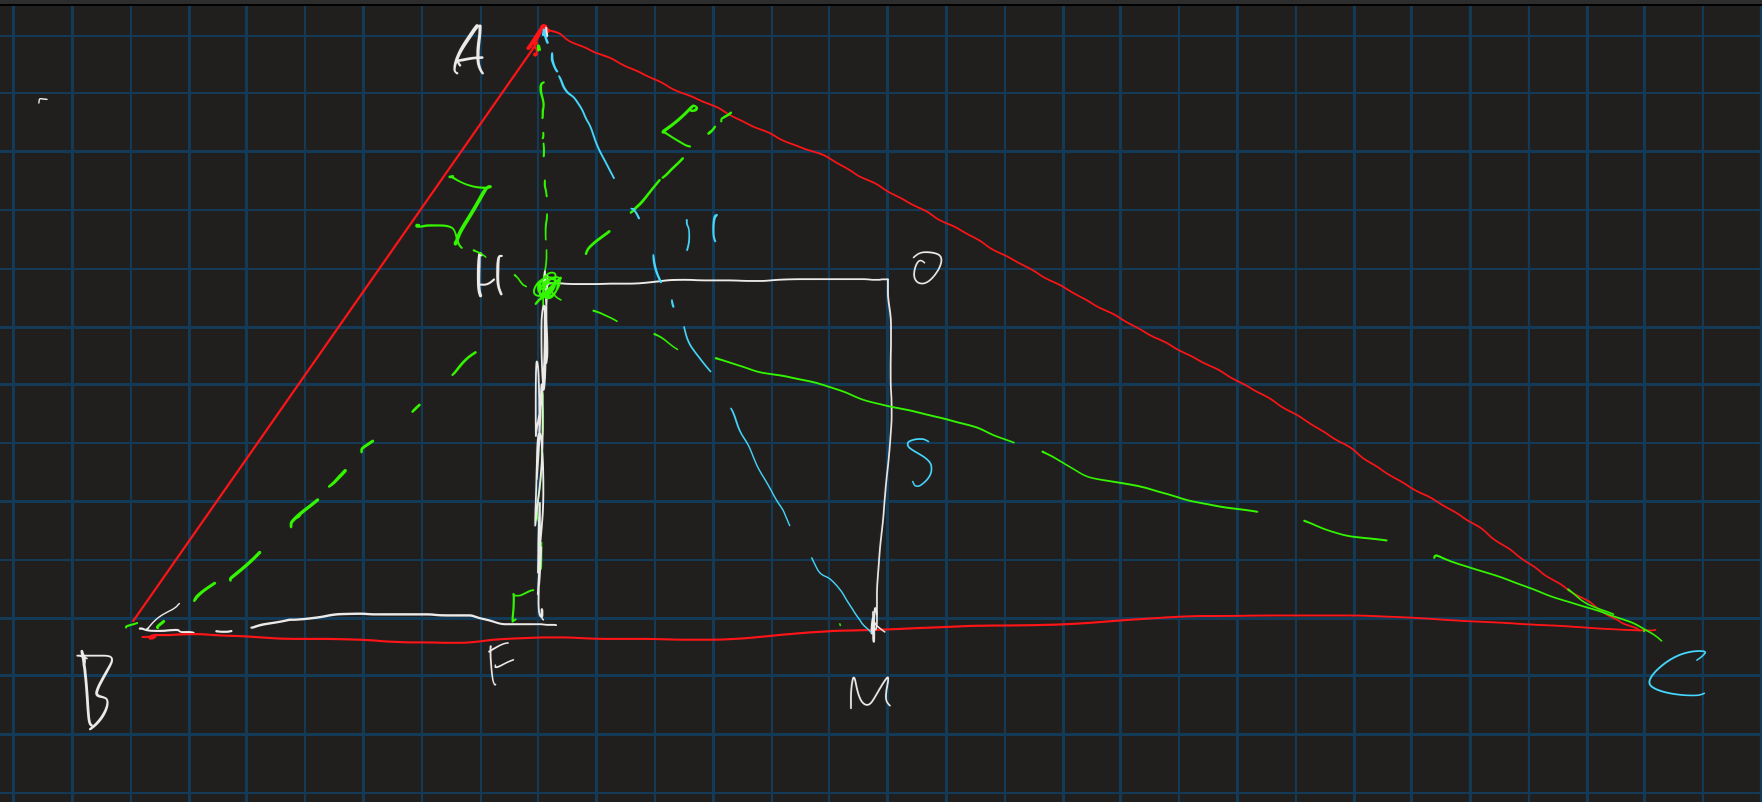
\includegraphics[scale=.5]{prob1}
  \begin{proof}
      \newcommand{\leng}[1]{\abs{\overline{#1}}}
      First consider the point $Z$ which is the centroid of of the triangle. We know that $Z$ is colinear to $H$ and $O$. This is noted because the centroid divides the medians into a $2:1$ ratio, and since $H$ and $O$ are colinear with $C$, that means $AH:HF$ has a $2:1$ ratio. Therefore \[\abs{\overline{AF}} = 3 \cdot \leng{HF} = 3 \cdot \leng{OM} = 15.\]
  
      We can also see that $\triangle BHF$ is similair to $\triangle ACF$, this gives us, \[\frac{\leng{BF}}{\leng{HF}} = \frac{\leng{AF}}{\leng{FC}} \rightarrow \leng{BF} \cdot \leng{FC} = \leng{AF} \cdot \leng{HF}  = 75. \]
  
      Now consider $\leng{BC}^{2}$, 
      \begin{align*}
          \leng{BC}^{2} &= (\leng{BF} + \leng{FC})^{2} \\
          &= (\leng{BF} - \leng{FC})^{2} + 4\leng{BF}\leng{FC} \\
          &= ((\leng{BM} - \leng{FM}) - (\leng{FM} + \leng{MC}))^{2} + 4\leng{BF}\leng{FC} \\
          &= (-2\leng{FM})^{2} + 4\leng{BF}\leng{FC} && \leng{BM} = \leng{MC} \\
          &= (2\leng{FM})^{2}+ 4\leng{BF}\leng{FC} .
      \end{align*}
  
      Solving for $\leng{BC}$, we get,
      \begin{align*}
          \leng{BC} &= \sqrt{(2\leng{FM})^{2}+ 4\leng{BF}\leng{FC}} \\
          &= \sqrt{22^{2} + 4(75)} \\
          &= 28.
      \end{align*}
  
      Thus the length of $\overline{BC}$ is 28.
  
  \end{proof}

\begin{tcolorbox}
    \begin{problem} {IC | 11/17 | 153.}
       Let $P$ be an arbitrary point in the interior of an equilateral triangle. Prove that the sum of the distances of P to the three sides is equal to the altitude of this triangle.
    \end{problem}
    \textbf{Geometry, Penultimate Step. } Used common geometric properties such as breaking up a shape and definition of altitude. Penultimate step came from realizing you need to connect the fact of equilateral triangle with altitude of the triangle 
\end{tcolorbox}
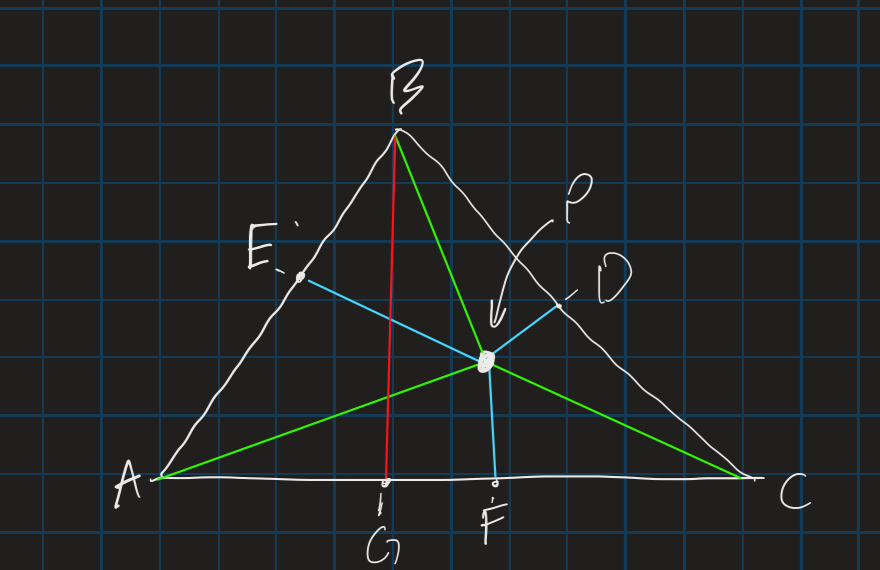
\includegraphics[scale= .5]{prob3}
\begin{proof} \newcommand{\leng}[1]{\abs{\overline{#1}}}
    First let us consider the area of the 3 triangles formed by $P$, 
    \begin{align*}
        [ABP] &= \frac{1}{2} \leng{AB} \cdot \leng{EP} \\
        [BCP] &= \frac{1}{2} \leng{BC} \cdot \leng{DP} \\
        [ACP] &= \frac{1}{2} \leng{AC} \cdot \leng{FP}
    \end{align*}

    These 3 triangles divide $\triangle ABC$ into 3 triangles, therefore the area of $\triangle ABC$ can be obtained by,
    \[[ABC] = [ABP] + [BCP] + [ACP]\]
    Recall though we are working with an equilateral triangle therefore all sides have the same length, which we can denote as $L$. This gives us,
    \begin{align*}
        [ABC] = \frac{1}{2} L \cdot (\leng{EP} + \leng{DP} +\leng{FP}).
    \end{align*}

    We also know though that the area of the triangle can be obtained by $[ABC] = \dfrac{1}{2} L \cdot \leng{BG}$. We see though $\overline{BG}$ is the altitude of the triangle, giving us, 
    \begin{align*}
        \frac{1}{2} L \cdot (\leng{EP} + \leng{DP} +\leng{FP}) &= \frac{1}{2} L \cdot \leng{BG} \\
        \leng{EP} + \leng{DP} +\leng{FP} &= \leng{BG}
    \end{align*}
    as desired.
\end{proof}

%--------------IC SUBMISSION-----------------------------

%--------------OC SUBMISSION-----------------------------
\begin{tcolorbox}
    \begin{problem} {OC 10/1 18}
        What is the first time the hour hand and minute hand meet after 1200?
    \end{problem}
    \textbf{Getting your hands dirty, Relax Conditions} This one was simply playing around with random times and seeing how the relation between the hour hand and minute hand changes. 
\end{tcolorbox}

\begin{solution}
    Since this is after 1200, that means the minute hand will be ahead of the hour hand for the first hour. It is not until 0100 that the minute hand will be at the 12th hour (0 degrees) position and the hour hand will be at the 1st hour (30 degrees). 

    Then with some simple math every minute that passes the minute hand moves 6 degrees while the hour hand moves 0.5 degrees. Using these facts we get the following,
    \begin{align*}
        0 + 6m &= 30 + 0.5m \\
        5.5m &= 30
    \end{align*}
    Solving for $m$ we get 5.45 minutes. Recall though the hour hand started at 1 (30 degrees). That means the first time they overlap after 1200 is 0105 or more specifically 1 hour, 5 minutes, and 27 seconds. 
\end{solution}

\begin{tcolorbox}
    \begin{problem} {OC - 10/25 - 61.}
        Show that $(n+1)^{n} \geq 2^{n}n!$
    \end{problem}
    \textbf{Pascal's triangle and binomial theorem, Inequalities} This one was kind of a straightforward induction step just utilizing properties listed. 
\end{tcolorbox}
\begin{proof}
    We will prove this using induction. 

    Case $n = 1$: \[(1+1)^{1} \geq 2^{1}1! \rightarrow 2 \geq 2\]

    Induction step, assume it holds for $n \geq k$.

    Case $n = k+1$:
    \begin{align*}
        (k+1)^{k} &\geq 2^{k}k! && \text{multiply by } 2(k+1) \\
        2(k+1)^{k+1} &\geq (k+1)!2^{k+1}
    \end{align*}
    The last thing we need is that we want to show $2(k+1)^{k+1} \leq (k+2)^{k+1}$ but this is of the form
    \begin{align*}
        2n^{n} &\leq (n+1)^{n} \\
        2 &\leq (1 + \frac{1}{n})^{n}
    \end{align*} 
    We know by binomial expansion that this does indeed hold though since the first two terms will be $1 + \frac{n}{n}$.
    Therefore it holds for $n = k+1$.
\end{proof}

\begin{tcolorbox}
    \begin{problem} {OC | 11/01 | 68}
        Imagine an $n \times n$ chessboard. How many ways is it possible to choose four squares, no three in the same row or columns which are the vertices of a rectangle?
    \end{problem}
    \textbf{Relax Conditions, Specialization} This one I was overthinking, and decided to try thinking about an 8x8 board specifically and then realized the key fact between the columns and rows.
\end{tcolorbox}
\begin{proof}
    If we have an $n\times n$ chessboard that means we have $n$ columns and $n$ rows. We can treat each row and column as sides of a rectangles. If we choose 2 unique vertical lines and 2 unique horizontal lines their intersections will generate a rectangle. There are n choose 2 ways to pick our horizontal lines, and n choose 2 ways to pick our vertical lines This means for an $n \times n$ chessboard we have, 
    \[\binom{n}{2}\binom{n}{2}\]
    rectangles
\end{proof}

\begin{tcolorbox}
    \begin{problem} {OC | 11/01 | 69.}
        A parking lot for compact cars has 12 adjacent spaces and eight are occupied. A large sport-utility vehicle arrives, needing two adjacent open spaces. What is the probability that it will be able to park?
    \end{problem}
    \textbf{Wishful thinking, Partitions and Bijections} Simply treating the SUV as a single parking spot and removing spaces accordingly made the problem easier
\end{tcolorbox}
\begin{proof}
    Consider the parking spaces to be the following squares, 
    \begin{align*}
        \square \square \square \square \square \square \square \square \square \square \square \square
    \end{align*}
    and our sport utility vehicle to be,
    \begin{align*}
        \boxtimes \boxtimes \boxtimes 
    \end{align*}
    Let us refer to the the vehicle's location by the left most box. So when we say the vehicle is at parking spot 1 it is the following,
    \begin{align*}
        \boxtimes \boxtimes \boxtimes \square \square \square \square \square \square \square \square \square
    \end{align*}
    and as it moves down we see we have to stop at the 10th parking spot because we get,
    \begin{align*}
        \square \square \square \square \square \square \square \square \square \boxtimes \boxtimes \boxtimes.
    \end{align*}

    We see in an empty parking lot we have 10 ways to part our vehicle. Meaning if 8 other vehicles came in after us they'd have 9 choose 8 ways to park with the remaining spots. This gives us $10 \cdot \binom{9}{8} = 90 $. So to get our probability we need to divide by all the ways the 8 cars can park in the 12 parking spots, in other words 12 choose 8 which is 495. Together this gives us,
    \begin{align*}
        \dfrac{90}{495} = \frac{2}{11} = .1818
    \end{align*}
    In other words we have an $18.18\%$ chance of finding parking for our vehicle. 
\end{proof}

\begin{tcolorbox}
    \begin{problem} {OC | 11/01 | 71.}
        How many ways are there to arrange 5 red balls, 7 green balls, and 9 blue balls in a line?
    \end{problem}
    \textbf{Get your hands dirty} Just a simple counting problem
\end{tcolorbox}
\begin{proof}
    First we can calculate the amount of ways we can put the balls in a line regardless of color, which is $21!$. Next lets consider the amount of ways we can arrange the red balls which is $5!$, then the amount of green balls which is $7!$, and finally the blue balls which is $9!$. The reason we want to do this is because we now need to take into account how many times each color appears in the line of balls to ultimately figure out how many ways we can line them up, since now all 21 balls are the same. This gives us,

    \begin{align*}
        \dfrac{21!}{5!7!9!} = 232792560
    \end{align*}
\end{proof}

\begin{tcolorbox}
    \begin{problem} {OC | 11/01 | 72.}
        How many ways are there to arrange 5 red balls, 7 green balls, and 9 blue balls in a line such that there are never two consecutive white balls?
    \end{problem}
    \textbf{Get your hands dirty} 
\end{tcolorbox}

\begin{proof}
    The problem mentions no white balls so I'm just going to choose how many ways are there such that there are never two consecutive blue balls.

    First we can line up the red and green balls to have a total line of 12 balls. Then we have 12 choose 7 ways to arrange the 7 green balls in this line of 12. This line of 12 will create 13 spaces, where 2 spaces at the ends of the line and 11 spaces between consecutive balls. This gives us 13 choose 9 ways to insert the blue balls into these spaces such that there are never 2 consecutive blue balls. This gives us,
    \[\binom{12}{7}\binom{13}{9} = 566280\]
\end{proof}

\begin{tcolorbox}
    \begin{problem} {OC | 11/03 | 77.}
        A poker hand consists of five cards. How many poker hands have a card from each of the four suits?
    \end{problem}
    \textbf{Get your hands dirty}
\end{tcolorbox}
\begin{proof}
    In this situation there has to be a suit that appears twice in the hand and the rest appear once. There are 4 ways to choose which suit will appear twice and then there are 13 choose 2 ways to pick 2 cards from the suit. Then there are 13 ways to pick a card for each of the remaining 3 suits. This gives us,
    \[4 \cdot \binom{13}{2} \cdot 13 \cdot 13 \cdot 13 = 685464. \]

    So there are 685464 hands that contain at least 1 of each suit.
\end{proof}

\begin{tcolorbox}
    \begin{problem} {OC | 11/08 | 83.}
        Prove that consecutive fibonacci nubers are relatively prime.
    \end{problem}
    \textbf{Recurrence relations, Primes and divisibility}
\end{tcolorbox}
\begin{proof}
    We know $F(1) = 1$ and $F(2) = 2$, thus, GCD$(F(1), F(2)) = 1$. 
    
    Assume that GCD$(F(n), F(n+1)) = 1$ holds.
    
    Now consider GCD$(F(n+1), F(n+2)) = $ GCD$(F(n+1), F(n+1) + F(n))$, but this is will be the same as GCD$(F(n+1), F(n))$, but from our induction step this is $1$.

    Therefore any two consecutive fibonacci terms are relatively prime.
\end{proof}

\begin{tcolorbox}
    \begin{problem} {OC | 11/12 | 90.}
        Prove there is a unique integer $n$ such that $2^{8} + 2^{11} + 2^{n}$ is a perfect square.
    \end{problem}
    \textbf{Get your hands dirty, Factor tactic}
\end{tcolorbox}
\begin{proof}
    This is similar to our IC class problem 143. First we see we are looking to satisfy the following,
    \begin{align*}
        2^{8} + 2^{11} + 2^{n} &= k^{2} \\
        2^{n} + 2304 &= k^{2} \\
        2^{n} &= k^{2} - 2304 \\
        2^{n} &= (k - 48)(k+48)
    \end{align*}

    Thus there has to be two powers of 2 such that their difference is 96. Consider 128, we see $128-96 = 32$, and botb $128$ and $32$ are powers of 2. This gives us the following,
    \[32 \cdot 128 = 2^{5} 2^{7} = 2^{12}.\]
    Therefore $n =12$ meaning there does exist indeed exist an $n$ such that the sum given is a perfect square.
\end{proof}


%--------------OC SUBMISSION-----------------------------

%--------------PP SUBMISSION-----------------------------

\begin{tcolorbox}
    \begin{problem} {IC | 11-22 | PP14}
        For which real numbers $c$ is there a straight line that intersects the curve \[x^{4} + 9x^{3} + cx^{2} + 9x + 4\]
        in four distinct points. 
    \end{problem}
    \textbf{Specialization, Polynomials}
\end{tcolorbox}
\begin{proof}
    We need this function to have two inflection points for then we know there is a line that will intersect it at 4 distinct points. To do this we have to look at its 2nd derivative which is,
    \[f''(x) = 12x^{2} + 54x + 2c.\]

    Now we need to solve for when the discriminant of the 2nd derivative is greater than zero, that way we have two distinct real roots. 
    \begin{align*}
        b^{2} - 4ac &> 0 \\
        54^{2} - 4\cdot12 \cdot 2c  > 0 \\
        2916 - 96c > 0 
    \end{align*}
    This is only true for $c \in (-\infty,30.375)$

\end{proof}

\begin{tcolorbox}
    \begin{problem} {IC | 11/29 | PP15}
        A square of side $2a$, always lying in the first quadrant, moves so that two consecutive vertices are always on the $x-$ and $y-$axes. Fin the locus of the center of the square.
    \end{problem}
    \textbf{Wishful thinking, Find and exploit symmetries}
\end{tcolorbox}
\begin{proof}
    The locus of the center of the square is clearly on the line $y = x$. Now we just need to find the minimum part of the line. This is when both vertices are on the same axis, say the y-axis. The center in which case is $(a,a)$. Now for the maximum. Continuing with the position mentioned, if the vertex at the origin begins to move to the right, and the vertex strictly on the on the y axis, the center reaches its maximum when the restricted vertices are placed at $(0,a)$ and $(a,0)$. This means are center will be $\sqrt{a^{2} + a^{2}} = \sqrt{2a^{2}} = \sqrt{2}a$ far from the origin. Thus the locus of the center of the square is on $y=x$ for $x \in [a, \sqrt{2}a]$
\end{proof}

\begin{tcolorbox}
    \begin{problem} {OC | 11/22 | PP 19}
        Find all ordered pairs $(a,b)$ of positive integers for which
        \[\frac{1}{a} + \frac{1}{b} = \frac{3}{2018}\]
    \end{problem}
    \textbf{Get your hands dirty, congruence, Factor Tactic} This problem was a messy one in that its a lot of computation, you do need to capitalize on congruence relations to learn about factors and find solutions from there. 
\end{tcolorbox}
\begin{proof}
    Let us manipulate the given equation,
    \begin{align*}
         2018\frac{1}{a} + 2018\frac{1}{b} &= 3 \\
         2018b + 2018a &= 3ab \\
         0 &= 3ab -2018a -2018b \\
         0 &= 9ab - (3)2018a - (3)2018b \\
         2018^{2} &= 9ab -(3)2018a - (3)2018b + 2018^{2} \\
         2018^{2} &= (3a-2018)(3b - 2018) && (1)
    \end{align*}

    We know $2018^{2} \equiv 1 \text{ mod }3$ therefore each factor in (1) most be congruent to $1$ mod $3$. The set of factors of $2018^{2}$ that are congruent to $1$ mod $3$ are,
    \[\set{2^{2}1009^{2}, 1009^{2}, 2^{2}1009, 1009, 2^{2}, 1} = X.\]
    Therefore we can determine the values of $a$ and $b$ by simply solving for $(3a - 2018) = x $ for $x \in X$. Calculating this, it gives us the following possible pairs which will satisfy the given equation,
    \[(674, 340033),\ (673, 1358114),\ (1009,2018), \ (2018,1009), \ (1358114, 673), \ (340033, 674)\] 
\end{proof}

\begin{tcolorbox}
    \begin{problem} {OC | 11/22 | PP 20.}
        Let $S$ be the smallest set of positive integers such that,
        \begin{itemize}
            \item[(a)] 2 is in $S$.
            \item[(b)] $n$ is in $S$ whenever $n^2$ is in $S$
            \item[(c)] $(n+5)^{2}$ is in $S$ whenever $n$ is in $S$  
        \end{itemize}
        what positive integers are not in $S$?
    \end{problem}
    \textbf{Get your hands dirty, Wishful thinking, Penultimate step} Had to play around with the fact that 2 is in the set to conclude what type of set is the smallest which give the penultimate step. 
\end{tcolorbox}
\begin{proof}
    Our claim is that,
    \begin{align*}
        S = \set{x \in \zz^{+} \mid x \neq 1,\ 5 \nmid x}
    \end{align*}
    in other words the integers $1$ and multiples of $5$ are not in $S$. First we will show that $S$ satisfies the 3 requirements. 

    For (a) it is obvious that $2 \neq 1$ and $5 \nmid 2$ therefore $S$ contains 2. 

    For (b) we know $5 \mid n^{2}$ if and only if $5 \mid n$. We also know $1^{2} = 1 \notin S$. Therefore for any $n^{2} \in S$ we have that $n \in S$.

    For (c) it follows simply from (b) since if $n \in S$ we have that $5\nmid n $ and therefore $5\nmid n+5$ which means $5 \nmid (n+5)^{2}$ thus $(n+5)^{2} \in S$.

    Now we just need to show that $S$ is indeed the smallest set of positive integers that satisfy these 3 requirements. We achieve this by showing if any other set, $S'$, satisfies these requirements then $S = S'$.

    Take $x \in S'$. Then by (c) $(x + 5)^{2} \in S'$ and by (b) we have $(n +5) \in S'$. We can note this consequence as, \[(*)\ \text{If }x \in S'  \rightarrow x+5k \in S', \ k \geq 0\] Now we know $2$ has to be in $S'$, which gives us the following implications,
    \begin{align}
        (2 + 5)^{2} = 49 &\in S' && \text{By (c)} \\
        (49 + 5)^{2} = (54)^{2} &\in S' && \text{By (c)} \\
        (54)^{2} + 5\cdot 44 = 56^{2} &\in S' && \text{By (*) where $k = 44$} \\
        56 &\in S' && \text{By (b)} \\
         56 + 5\cdot 13 = 121 &\in S' && \text{By (*) where $k = 13$} \\
         121 = 11^{2}, \ 11 &\in S' && \text{By (b)} \\
         11 + 5 = 16 &\in S' && \text{By (*) where $k = 1$} \\
         16 = 4^{2}&\in S' && \text{By (b)} \\
         4 + 5 = 9 &\in S' && \text{By (*)} \\
         9 = 3^{2} &\in S' && \text{By (b)}  
    \end{align}

    What we want to take away from these implications is that because $2$ is in $S'$ then so are $3,4$. Now let us resume from the fact that $16 \in S'$ which we know from line (7),
    \begin{align}
        16 + 5 \cdot 4 = 36 &\in S' && \text{By (*) where $k = 4$} \\
        36 = 6^{2}, \ 6 &\in S' && \text{By (b)}
    \end{align}

    Now we know that if a set $S'$ satisfies the 3 requirements then we know $2,3,4,6 \in S'$ then by applying $(*)$ to each of these values for all $k\geq 0$,
    \begin{align*}
        S' = \set{x \in \zz^{+}\mid x \neq 1, \ 5 \nmid x}
    \end{align*}
    which means $S = S'$, therefore $S$ is indeed the smallest set of positive integers satisfying these requirements.
\end{proof}

\begin{tcolorbox}
    \begin{problem} {IC | 11/29 | PP 28}
        Determine all possible values of $A^{3} + B^{3} + C^{3} - 3ABC$ where $A,B,C \in \nn_0$
    \end{problem}
    \textbf{Congruence, Inequalities, Arithmetic and geometric sequences and series, Get your hands dirty, Factor tactic}
\end{tcolorbox}
\begin{proof}
    Let $A^{3} + B^{3} + C^{3} -3ABC = D$. Our claim is that $D$ can be any nonnegative integer except multiplies of 3 which are not multiples of 9. Now without loss of generality we can let $A$ be the smallest of the 3 nonnegative integers we input into the equation for $(A,B,C)$. Now let $c,b \in \nn_0$, this lets us express $C$ and $B$ as, $C = A + c$ and $B = A + b$,
    \begin{align*}
        D &= A^{3} + B^{3} + C^{3} -3ABC  \\
        D &= A^{3} + (A+b)^{3} + (A + c)^{3} - 3A(A+b)(A+c)  \\
    \end{align*}
    after expanding out we get,
    \begin{align*}
        D &= (3A + b + c)(b^{2} -bc + c^{2}) 
    \end{align*}
    If we let $(b,c) = (0,1)$ we get $D = 3A + 1$. So as $A$ varies in $\nn_0$ we get every nonnegative integer congruent to 1 mod 3. 

    If we let $(b,c) = (1,1)$ we get $D = 3A + 2$. So as $A$ varies in $\nn_0$ we get every nonnegative integer congruent to 2 mod 3.

    If we let $(b,c) = (1,2)$ we get $D = 9A + 9$. So as $A$ varies in $\nn_0$ we get every multiple of 9 except 0. 

    Finally $D$ is equal to 0 when $A = 0 = b = c$. Now all we need to show is that $D$ can't be any value other than the ones claimed above. 

    First we know that $D$ must be nonnegative because (AM-GM inequality),
    \begin{align*}
        \frac{A^{3} + B^{3} + C^{3}}{3} \geq \sqrt[3]{A^{3}B^{3}C^{3}} \\
        \frac{A^{3} + B^{3} + C^{3}}{3} \geq  ABC \\
        A^{3} + B^{3} + C^{3} \geq 3ABC
    \end{align*}

    Now we must show if $D$ is a multiple of $3$ then it has to be a multiple of 9. Consider the following. 
    \begin{align*}
        D &= (3A + b + c)(b^{2} - bc + c^{2}) \\
        D &= (3A + (b + c))((b+c)^{2}-3bc) && (1) \\
        D &= 3A(b+c)^{2} + (b+c)^{3} -9Abc -3bc(b+c) \\
        D &= 3(A(b+c)^{2} -3Abc -bc(b+c)) + (b+c)^{3} && (2)
     \end{align*}
     We know then from $(2)$ that,
     \begin{align*}
         D \equiv (b+c)^{3} \equiv (b+c) \text{ mod } 3
     \end{align*}
     As a consequence if $D$ is divisible by 3, then $(b+c)$ must also be divisible by 3 meaning each factor in $(1)$ is divisible by 3 and as a result $D$ must be divisible by 9, as desired.
\end{proof}

\begin{tcolorbox}
    \begin{problem} {IC | 12/01 | PP 36}
        Basketball star Shanille O'Keal's team statistician keeps track of the number, $S(N)$, of successful free throws she has made in her first $N$ attempts of the season. Early in the season, $S(N)$ was less than $80\%$ of $N$, but by the end of the season, $S(N)$ was more than $80\%$ of $N$. Was there necessarily a moment in between when $S(N)$ was exactly $80\%$ of $N$?
    \end{problem}
    \textbf{Inequalities, Get your hands dirty}
\end{tcolorbox}
\begin{proof}
    We will prove this by contradiction, let us assume that there was not a moment when $S(N) = 80\%$. That means there was an $n \in \nn$ such that $S(n) < 80\%$ and $S(n +1) > 80\%$. Let $k\in \nn_0$ be the number of successful free throws of the $n$ attempts, that means,
    \begin{align*}
        S(n) < 80\% &\rightarrow \frac{k}{n} < \frac{4}{5} \rightarrow 5k < 4n &&(1)\\
        S(n+1) > 80\% &\rightarrow \frac{k+1}{n+1} > \frac{4}{5} \rightarrow  5k +1 > 4n && (2) 
    \end{align*}
    Putting (1) and (2) together we get,
    \begin{align*}
        5k < 4n < 5k+1
    \end{align*}
    The inequality above gives us a contradiction though since $5k$ and $5k+1$ are positive consecutive integers, and $4n$ is a positive integer which means it can't be strictly between $5k$ and $5k +1$. Therefore there must be a moment where $S(N)$ was exactly $80 \%$.
\end{proof}

\begin{tcolorbox}
    \begin{problem} {OC | 10/15 | 37 (Putnam)}
        Prove that there exist infinitely many integers $n$ such that $n,n+1,n +2$ are each the sum of the squares of two integers. 
    \end{problem}
    \textbf{Penultimate step, Factor tactic} This one once you really think about what you need to show you can can in a way "Force" a discovery of such an $n$ by kind of working backwards and taking advantage of factors
\end{tcolorbox}
\begin{proof}
    Let $k \in \zz$, then let $n = (2k^{2} + 1)^{2} -1$. We see we can express $n$ as the sum of the squares of two integers through the following,
    \begin{align*}
       n =  (2k^{2}+1)^{2} -1 &= (2k^{2} + 1)(2k^{2} + 1) -1 \\
        &= 4k^{4} +2k^{2} + 2k^{2} + 1 -1 \\
        &= 4k^{4} + 4k^{2} \\
        &= (2k^{2})^{2} + (2k)^{2}
    \end{align*}

    For $n+1$,
    \begin{align*}
         n +1 = (2k^{2} + 1)^{2} -1 + 1 = (2k^{2} + 1)^{2} + 0^{2}
    \end{align*}
    
    For $n+2$, 
    \begin{align*}
        n +2 = (2k^{2} +1)^{2} -1 + 2 = (2k^{2} +1)^{2} + 1^{2}
    \end{align*}
    Since $k \in \zz$, that means there is indeed an infinite number of $n$ that satisfy the given statement.
\end{proof}

\begin{tcolorbox}
    \begin{problem} {IC | 12-03 | PP 40}
        A right circular cone has base of radius 1 and height 3. A cube is inscribed in the cone so that one face of the cube is contained in the base of the cone. What is the side length of the cube?
    \end{problem}
    \textbf{Find and exploit symmetries, Geometry}
\end{tcolorbox}
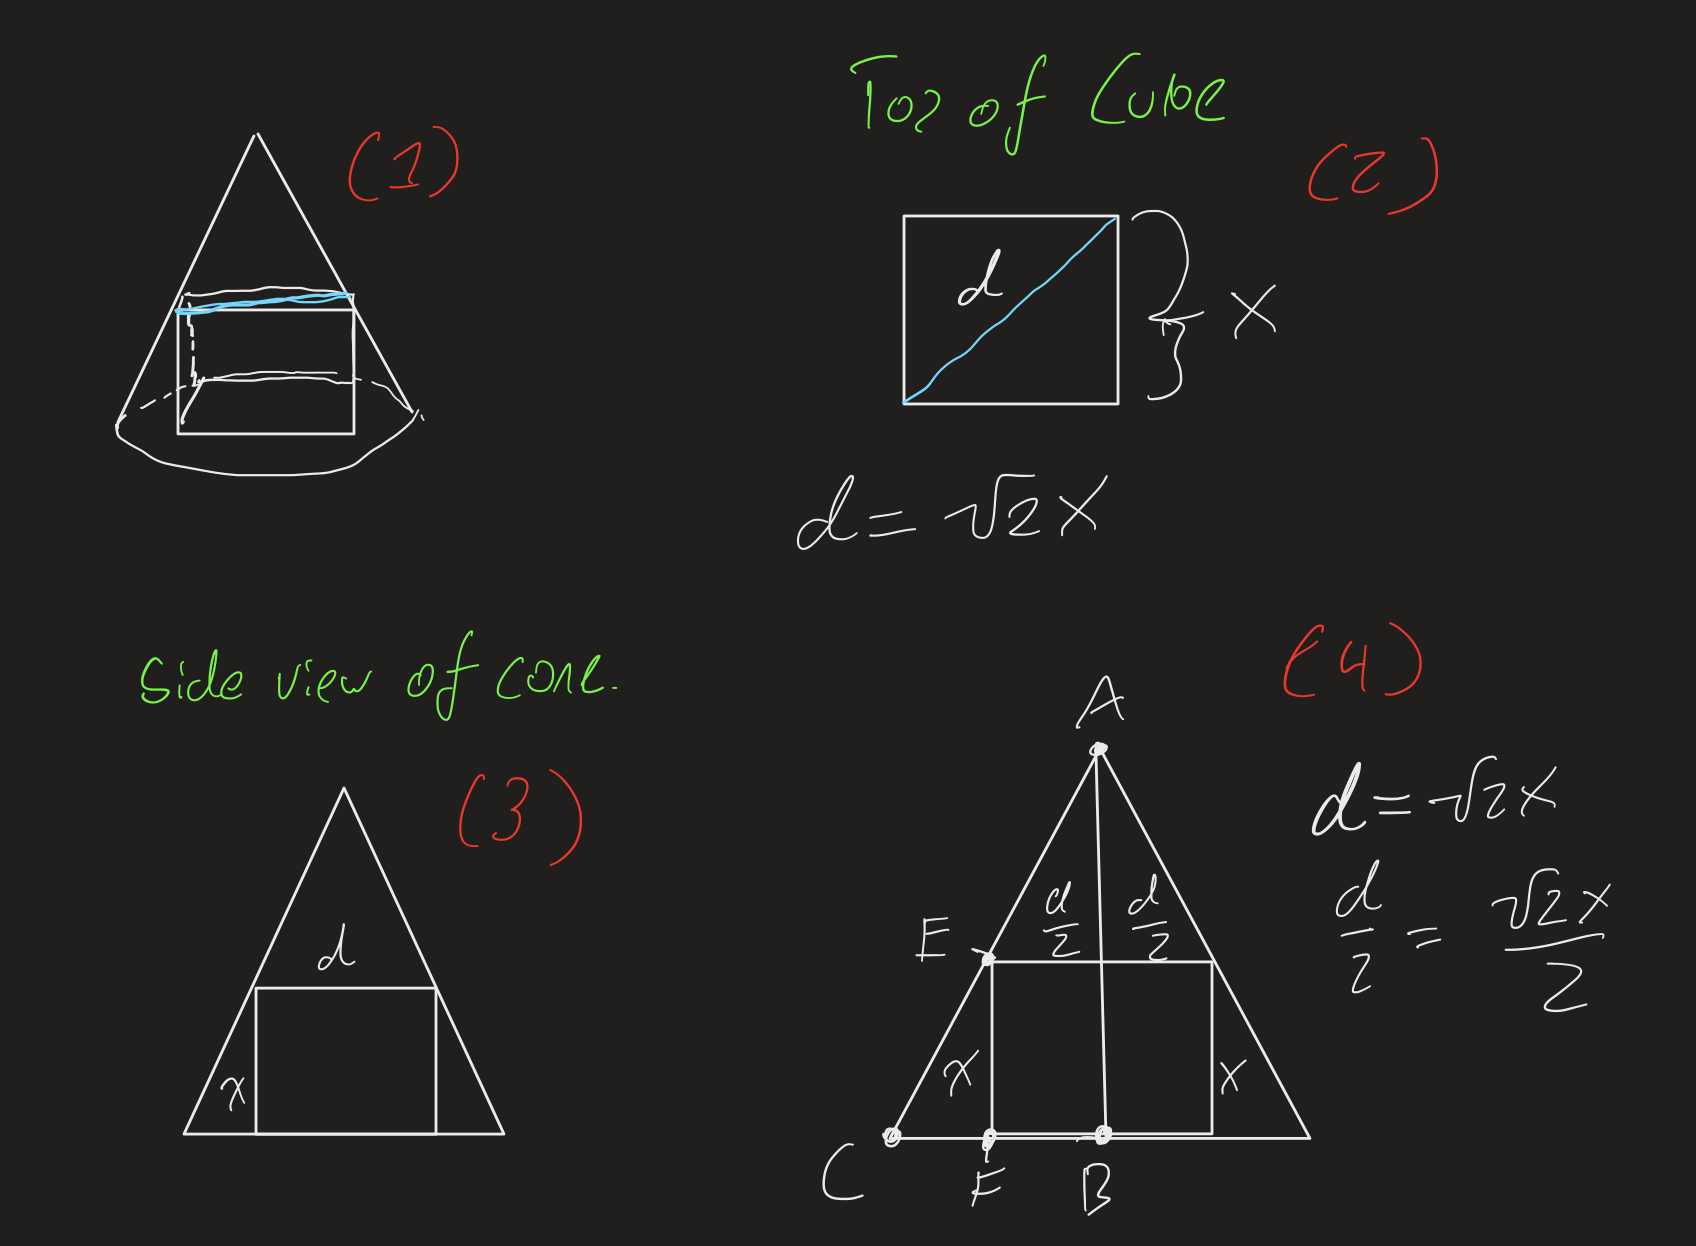
\includegraphics[scale=0.5]{diagram}
\begin{proof}
    Consider the cube inscribed in a cone as in image (1), where the lengths of each side are denoted by $x$, and the diagonal of the top of the cube is denoted by $d$ as seen in (2). We know that $d = \sqrt2 x$. Now consider the side view of the cone such that our view is perpendicular to the top diagonal of the square, giving us a triangle as seen in (3). We can bisect this triangle perpendicular to its base to obtain two more triangles as seen in (4). Each of these new triangles will then have a rectangle of side lengths $x$ and $\frac{d}{2}$ inside of them. We see that the triangle formed by $\triangle ABC$ is similar to $\triangle CEF$. This gives us the following equation,
    \begin{align*}
        \frac{1}{3} = \frac{1-\frac{d}{2}}{x} = \frac{1- \frac{\sqrt2 x}{2}}{x}
    \end{align*}
    now let's solve for $x$,
    \begin{align*}
        x &= 3 - \frac{3\sqrt2 x}{2}\\
        x + \frac{3\sqrt2 x}{2} &= 3 \\
        x(1 + \frac{3\sqrt 2}{2}) &= 3 \\
        x &= \frac{3}{1 + \frac{3\sqrt2}{2}} \approx 0.9661
    \end{align*}
\end{proof}

\begin{tcolorbox}
    \begin{problem} {IC | 12/03 | PP 41.}
        Find the minimum value of $\dfrac{(x+\frac{1}{x})^{6} - (x^{6}+\frac{1}{x^{6}}) -2)}{(x+\frac{1}{x})^{3} + (x^{3} + \frac{1}{x^{3}})}$ for $x > 0$
    \end{problem}
    \textbf{Factor Tactic, Get your hands dirty, wishful thinking} Using factors to help simplify the equation and express the equation in a cleaner way through wishful thinking. This was only seen though after playing around with the equation until I saw the desired expression 
\end{tcolorbox}
\begin{proof}
    First let us manipulate the numerator of the given equation so that we can substitute $x + \frac{1}{x}$ with $y$.
    \begin{align*}
        (x+\frac{1}{x})^{6} - (x^{6} + \frac{1}{x^{6}}) -2 &= (x+ \frac{1}{x})^{6} - (x^{2} + \frac{1}{x^{2}})(x^{4} + \frac{1}{x^{4}} - 1) - 2 \\
        &= (x + \frac{1}{x})^{6} - ((x + \frac{1}{x})^{2}-2)((x^{2} + \frac{1}{x^{2}})^{2} - 3) - 2 \\
        &= (x + \frac{1}{x})^{6} - ((x + \frac{1}{z})^{2} - 2)(((x + \frac{1}{x})^{2} - 2)^{2} -3) - 2 \\
        &= y^{6} - (y^{2} - 2)((y^{2}-2)^{2} - 3) - 2 \\
        &= y^{6} - (y^{2} - 2)(y^{4}-4y^{2} + 1) -2 \\
        &= 4y^{2} - y^{2} + 2y^{4} -8y^{2} \\
        &= 6y^{4} - 9y^{2} && (1)
    \end{align*}
    Now let us do the same for the denominator of the given equation.
    \begin{align*}
        (x + \frac{1}{2})^{3} + (x + \frac{1}{x})(x^{2} + \frac{1}{x^{2}} -1) &= (x + \frac{1}{x'})^{3} + (x + \frac{1}{x})((x + \frac{1}{x})^{2} - 3) \\
        &= y^{3} + y(y^{2} - 3) \\
        &= 2y^{3} - 3y && (2)
    \end{align*}
    (1) and (2) together means,
    \begin{align*}
        \dfrac{(x+\frac{1}{x})^{6} - (x^{6}+\frac{1}{x^{6}}) -2)}{(x+\frac{1}{x})^{3} + (x^{3} + \frac{1}{x^{3}})} = \frac{6y^{4} - 9y^{2}}{2y^{3} - 3y} &= 3y \\ 
        &= 3(x + \frac{1}{x})
    \end{align*}
    We know though for $x > 0$ that $(x + \frac{1}{x})$ is bounded below by $2$, therefore,
    \begin{align*}
        3(x + \frac{1}{x}) \geq 3\cdot 2 = 6
    \end{align*}
    So $6$ is the minimum value of the given equation for $x> 0$
\end{proof}

\begin{tcolorbox}
    \begin{problem} {IC | 12-03 | PP 42}
      Let $k > 1$ be a positive integer. Show that the equation $x^{2} -y^{2} = k^{3}$
  always has integral solutions in $x$ and $y$.
    \end{problem}
    \textbf{Diophantine equation, Factor tactic, Primes and divisibility} Once you see you can create an expression with $k$ that will be even it allows for one to solve for the system of equations which can be found through factoring
  \end{tcolorbox}
  \begin{proof}
      Consider the following,
      \begin{align*}
          x^{2} - y^{2} &= k^{3} \\
          (x+y)(x-y) &= (k^{2})(k) && (1)
      \end{align*}
      (1) gives us the system of equations,
      \begin{align*}
          (x+y) &= k^{2} \\
          (x-y) &= k.
      \end{align*}
      We know that $k^{2} - k$ and $k^{2} +k $ will yield an even integer for any $k \in \zz$. This allows us to set $x = \frac{k^{2} + k}{2}$ and $y = \frac{k^{2} - k}{2}$. We see then,
      \begin{align*}
          (x+y)(x-y) &= (\frac{k^{2} + k}{2} + \frac{k^{2} - k}{2})(\frac{k^{2} + k}{2} -\frac{k^{2} - k}{2}) \\
          &= \frac{2k^{2}}{2}\frac{2k}{2} \\
          &= k^{2}k\\
          &= k^{3}
      \end{align*}
      meaning $x^{2}-y^{2} = k^{3}$ always has integral solutions in $x$ and $y$, by simply setting $x = \frac{k^{2} + k}{2}$ and $y = \frac{k^{2} - k}{2}$.
    \end{proof}

%--------------PP SUBMISSION-----------------------------

\end{document}